\documentclass[journal,12pt,twocolumn]{IEEEtran}

\usepackage{setspace}
\usepackage{gensymb}

\singlespacing


\usepackage[cmex10]{amsmath}

\usepackage{amsthm}

\usepackage{mathrsfs}
\usepackage{txfonts}
\usepackage{stfloats}
\usepackage{bm}
\usepackage{cite}
\usepackage{cases}
\usepackage{subfig}

\usepackage{longtable}
\usepackage{multirow}

\usepackage{enumitem}
\usepackage{mathtools}
%\usepackage{steinmetz}
\usepackage{tikz}
\usepackage{circuitikz}
\usepackage{verbatim}
%\usepackage{tfrupee}
\usepackage[breaklinks=true]{hyperref}

\usepackage{tkz-euclide}

\usetikzlibrary{calc,math}
\usepackage{listings}
    \usepackage{color}                                            %%
    \usepackage{array}                                            %%
    \usepackage{longtable}                                        %%
    \usepackage{calc}                                             %%
    \usepackage{multirow}                                         %%
    \usepackage{hhline}                                           %%
    \usepackage{ifthen}                                           %%
    \usepackage{lscape}     
\usepackage{multicol}
\usepackage{chngcntr}

\DeclareMathOperator*{\Res}{Res}

\renewcommand\thesection{\arabic{section}}
\renewcommand\thesubsection{\thesection.\arabic{subsection}}
\renewcommand\thesubsubsection{\thesubsection.\arabic{subsubsection}}

\renewcommand\thesectiondis{\arabic{section}}
\renewcommand\thesubsectiondis{\thesectiondis.\arabic{subsection}}
\renewcommand\thesubsubsectiondis{\thesubsectiondis.\arabic{subsubsection}}


\hyphenation{op-tical net-works semi-conduc-tor}
\def\inputGnumericTable{}                                 %%

\lstset{
%language=C,
frame=single, 
breaklines=true,
columns=fullflexible
}
\begin{document}


\newtheorem{theorem}{Theorem}[section]
\newtheorem{problem}{Problem}
\newtheorem{proposition}{Proposition}[section]
\newtheorem{lemma}{Lemma}[section]
\newtheorem{corollary}[theorem]{Corollary}
\newtheorem{example}{Example}[section]
\newtheorem{definition}[problem]{Definition}

\newcommand{\BEQA}{\begin{eqnarray}}
\newcommand{\EEQA}{\end{eqnarray}}
\newcommand{\define}{\stackrel{\triangle}{=}}
\bibliographystyle{IEEEtran}
\providecommand{\mbf}{\mathbf}
\providecommand{\pr}[1]{\ensuremath{\Pr\left(#1\right)}}
\providecommand{\qfunc}[1]{\ensuremath{Q\left(#1\right)}}
\providecommand{\sbrak}[1]{\ensuremath{{}\left[#1\right]}}
\providecommand{\lsbrak}[1]{\ensuremath{{}\left[#1\right.}}
\providecommand{\rsbrak}[1]{\ensuremath{{}\left.#1\right]}}
\providecommand{\brak}[1]{\ensuremath{\left(#1\right)}}
\providecommand{\lbrak}[1]{\ensuremath{\left(#1\right.}}
\providecommand{\rbrak}[1]{\ensuremath{\left.#1\right)}}
\providecommand{\cbrak}[1]{\ensuremath{\left\{#1\right\}}}
\providecommand{\lcbrak}[1]{\ensuremath{\left\{#1\right.}}
\providecommand{\rcbrak}[1]{\ensuremath{\left.#1\right\}}}
\theoremstyle{remark}
\newtheorem{rem}{Remark}
\newcommand{\sgn}{\mathop{\mathrm{sgn}}}
\providecommand{\abs}[1]{\left\vert#1\right\vert}
\providecommand{\res}[1]{\Res\displaylimits_{#1}} 
\providecommand{\norm}[1]{\left\lVert#1\right\rVert}
%\providecommand{\norm}[1]{\lVert#1\rVert}
\providecommand{\mtx}[1]{\mathbf{#1}}
\providecommand{\mean}[1]{E\left[ #1 \right]}
\providecommand{\fourier}{\overset{\mathcal{F}}{ \rightleftharpoons}}
%\providecommand{\hilbert}{\overset{\mathcal{H}}{ \rightleftharpoons}}
\providecommand{\system}{\overset{\mathcal{H}}{ \longleftrightarrow}}
	%\newcommand{\solution}[2]{\textbf{Solution:}{#1}}
\newcommand{\solution}{\noindent \textbf{Solution: }}
\newcommand{\cosec}{\,\text{cosec}\,}
\providecommand{\dec}[2]{\ensuremath{\overset{#1}{\underset{#2}{\gtrless}}}}
\newcommand{\myvec}[1]{\ensuremath{\begin{pmatrix}#1\end{pmatrix}}}
\newcommand{\mydet}[1]{\ensuremath{\begin{vmatrix}#1\end{vmatrix}}}
\numberwithin{equation}{subsection}
\makeatletter
\@addtoreset{figure}{problem}
\makeatother
\let\StandardTheFigure\thefigure
\let\vec\mathbf
\renewcommand{\thefigure}{\theproblem}
\def\putbox#1#2#3{\makebox[0in][l]{\makebox[#1][l]{}\raisebox{\baselineskip}[0in][0in]{\raisebox{#2}[0in][0in]{#3}}}}
     \def\rightbox#1{\makebox[0in][r]{#1}}
     \def\centbox#1{\makebox[0in]{#1}}
     \def\topbox#1{\raisebox{-\baselineskip}[0in][0in]{#1}}
     \def\midbox#1{\raisebox{-0.5\baselineskip}[0in][0in]{#1}}
\vspace{3cm}
\title{EE5609 Assignment 5}
\author{SHANTANU YADAV, EE20MTECH12001 }
\maketitle
\newpage
\bigskip
\renewcommand{\thefigure}{\theenumi}
\renewcommand{\thetable}{\theenumi}

The python solution code is available at
\begin{lstlisting}
https://github.com/Shantanu2508/Matrix_Theory/blob/master/Assignment_5/assignment5.py
\end{lstlisting}

\section{Problem}
Prove that the equation
\begin{align*}
	12x^2 + 7xy -10y^2 +13x +45y -35 =0 
\end{align*}
represents two straight lines and find the angle between the lines.
\section{Solution}
The above equation can be expressed as
\begin{align}
        \vec{x}^{T}\vec{Vx} + 2\vec{u}^{T}\vec{x} + f=0   \label{eq2}
\end{align}
where
\begin{align}
	\vec{V}=\vec{V}^T &= \myvec{12 & \frac{7}{2} \\ \frac{7}{2} & -10} \\
	\vec{u} &= \myvec{\frac{13}{2} \\ \frac{45}{2}} \\
	 f=-35
\end{align}	
	(\ref{eq2}) represents a pair of straight lines if
\begin{align}
	&\mydet{\vec{V} & \vec{u} \\ \vec{u}^T & f} = 0     \label{eq5} \\
	\mydet{\vec{V} & \vec{u} \\ \vec{u}^T & f} 
		&= \mydet{12 & \frac{7}{2}  & \frac{13}{2} \\ 
	        \frac{7}{2} & -10 & \frac{45}{2}     \\
	       \frac{13}{2} & \frac{45}{2} & -35 }  \\
	       		\nonumber \\
	\implies \ 12\mydet{-10 & \frac{45}{2} \\ \frac{45}{2} & -35} 
		& -\frac{7}{2}\mydet{\frac{7}{2} & \frac{45}{2} \\ \frac{13}{2} & -35} 
		+\frac{13}{2}\mydet{\frac{7}{2} & -10 \\ \frac{13}{2} & \frac{45}{2}} = 0 \label{eq10}\\
\end{align}
The lines intercept if
\begin{align}
        \mydet{\vec{V}} < 0
 	\mydet{\vec{V}}=-\frac{529}{4} < 0 \label{eq11}
\end{align}
From (\ref{eq10}) and (\ref{eq11}) it can be concluded that the given equation represents a pair of intersecting lines.
Let the equations of lines be
\begin{align}
	\vec{n_1}^T \vec{x}=c_1 \\
	\vec{n_2}^T \vec{x}=c_2 
\end{align}
Since (\ref{eq2}) represents a pair of straight lines it must satisfy
\begin{align}
	(\vec{n_1}^T \vec{x} - c_1)(\vec{n_1}^T \vec{x} - c_1) =
        \vec{x}^{T}\vec{Vx} + 2\vec{u}^{T}\vec{x} + f=0
\end{align}
where
\begin{align}
	\vec{n_1}*\vec{n_2}=\myvec{a\\2b\\c}=\myvec{12\\7\\-10} \label{eq6} \\ 
	c_2\vec{n_1}+c_1\vec{n_2}=-2\vec{u} \label{eq9}\\
	c_1c_2=f
\end{align}
Slopes of the lines can be obtained by solving 
\begin{align}
	cm^2+2bm+a=0 \\
	-10m^2+7m+12=0 \\
	\implies m_1 = \frac{-4}{5}, m_2 = \frac{3}{2}
\end{align}
The normal vectors can be expressed in terms of corresponding slopes of lines as
\begin{align}
	\vec{n}=k\myvec{-m\\1} \\
	\implies
	\vec{n_1}=k_1\myvec{\frac{4}{5} \\ 1}  \label{eq7} \\
	\vec{n_2}=k_2\myvec{-\frac{3}{2} \\ 1}  \label{eq8}
\end{align}
Substituing (\ref{eq7}) and (\ref{eq8}) in (\ref{eq6}) we get
\begin{align}
	k_1k_2=-10
\end{align}
Assuming $ k_1=5$ and $k_2 =-2$
\begin{align}
	\vec{n_1}=\myvec{4\\5}, \vec{n_2}=\myvec{3\\-2}
\end{align}
Verification using Toeplitz matrix
\begin{align}
\vec{n_1}*\vec{n_2}=\myvec{4 & 0 \\ 5 & 4 \\0 & 5}\myvec{3\\-2}=\myvec{12\\7\\-10}
\end{align}
From (\ref{eq9}) we have
\begin{align}
	c_2\myvec{4\\5}+c_1\myvec{3\\-2}=\myvec{-13\\-45}
\end{align}
Solving the augmented matrix
\begin{align}
	\myvec{4 & 3 & -13 \\ 5 & -2 & -45}
	\xleftrightarrow[]{R_2 \leftarrow 4R_2-5R_1}
	\myvec{4 & 3 & -13 \\ 0 & -23 & -115}\\
	\xleftrightarrow[]{R_2 \leftarrow -\frac{R_2}{23}}
        \myvec{4 & 3 & -13 \\ 0 & 1 & 5}
        \xleftrightarrow[]{R_1 \leftarrow R_1-3R_2}
	\myvec{4 & 0 & -28 \\ 0 & 1 & 5}\\
	\xleftrightarrow[]{R_1 \leftarrow \frac{R_1}{4}}
        \myvec{1 & 0 & -7 \\ 0 & 1 & 5} \\
	\implies \quad c_1 =-7, \ c_2 =5
\end{align}
Thus the equation of lines are
\begin{align}
	\myvec{4 & 5}\vec{x} = 5 \\
	\myvec{3 & -2}\vec{x} = -7 
\end{align}
The angle between the lines can be expressed interms of normal vectors 
\begin{align}
	\vec{n_1}=\myvec{4\\5} , \quad \vec{n_2}=\myvec{3\\-2}
\end{align}
as
\begin{align}
	\cos\theta=\frac{\vec{n_1}^T\vec{n_2}}{\norm{\vec{n_1}}\norm{\vec{n_2}}} \\
				\nonumber \\
	\implies \quad \theta=\cos^{-1}({\frac{2}{\sqrt{533}}}) = \tan^{-1}(\frac{23}{2})
\end{align}
\begin{figure}[!h]
	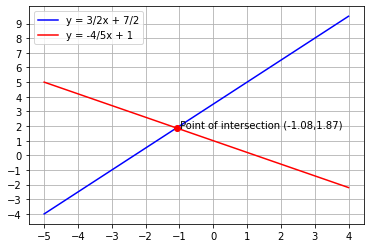
\includegraphics[width=\columnwidth]{lines.png}
	\caption{} \label{linefig1}
\end{figure}
\end{document}
